\chapter{Redes neuronales y YOLO sin complicaciones}

\begin{enpocas}
Qué es aprender con ejemplos, cómo funciona una neurona, qué es una convolución, cómo detecta objetos
YOLO y cómo se mide si funciona: IoU, precisión, recall y mAP.
\end{enpocas}

\section{Programar contra aprender}

Escribir reglas para reconocer a una persona desde el aire (``un grupo de píxeles de color piel...'')
falla de inmediato: hay ropa de todos colores, sombras, personas acostadas o tapadas por ramas. El
\textbf{aprendizaje automático} hace lo contrario: se le dan miles de imágenes con la respuesta correcta
y el programa ajusta sus parámetros hasta acertar.

\section{La neurona artificial}

Una neurona multiplica cada entrada por un \textbf{peso}, suma todo con un \textbf{sesgo} y pasa el
resultado por una función de activación:
\begin{equation}
y = \text{activación}\Big(\sum_i w_i x_i + b\Big).
\end{equation}
Muchas neuronas en capas forman una \textbf{red}. Entrenar es encontrar los pesos que hacen que la red
acierte. La misma idea sirve para ver (YOLO) y para controlar (la red 15-64-32-4 del
capítulo~\ref{cap:control-neuronal}).

\section{Convoluciones}

Las redes para imágenes usan \textbf{convoluciones}: filtros pequeños que se deslizan por la imagen
buscando patrones locales (bordes, texturas, formas). Las primeras capas detectan bordes; las
siguientes, partes; las últimas, objetos completos. Los filtros no se diseñan: se aprenden.

\begin{figure}[H]
\centering
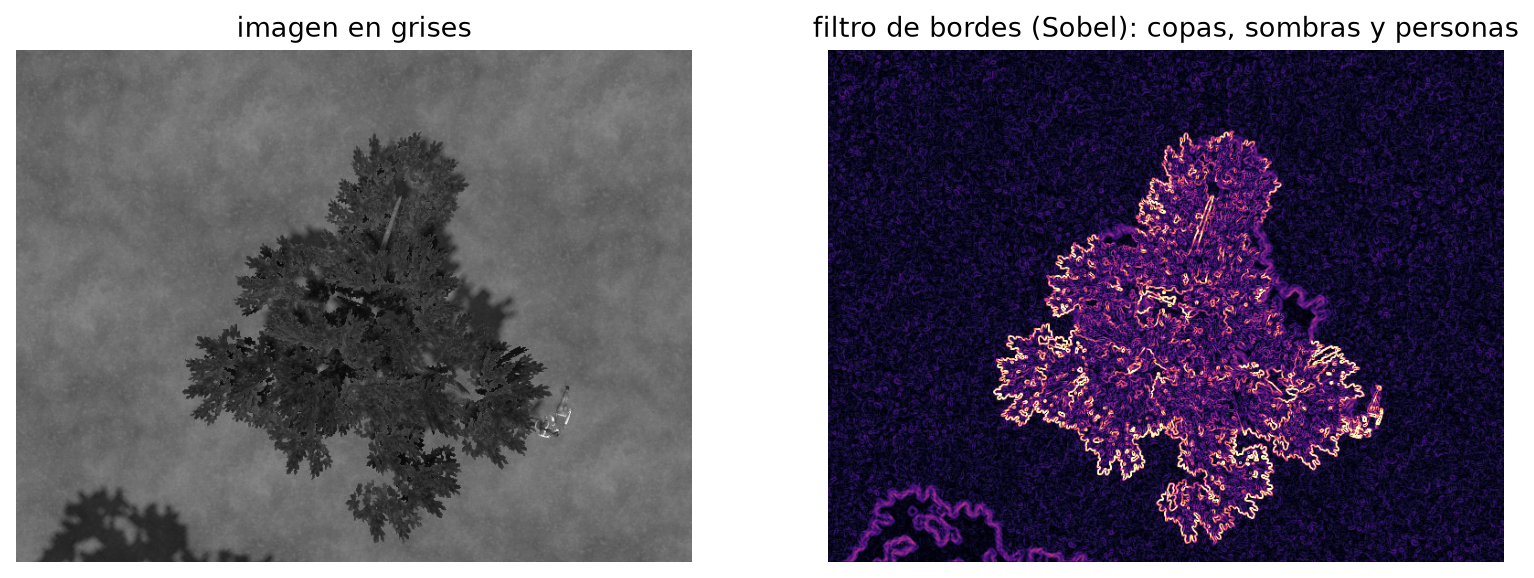
\includegraphics[width=\textwidth]{convolucion_personas.png}
\caption{Un filtro de bordes aplicado a una imagen del dron: resalta copas, sombras y personas.}
\end{figure}

\section{YOLO}

\textbf{YOLO} (\emph{You Only Look Once}) predice en una sola pasada todos los recuadros de la imagen,
cada uno con su clase y su confianza. Usamos \textbf{YOLO26s}, la versión vigente de Ultralytics en
tamaño \emph{small}: la \emph{nano} es más rápida pero pierde personas pequeñas. Procesa una imagen de
1280 píxeles en $\approx$16~ms en la GPU.

\begin{figure}[H]
\centering
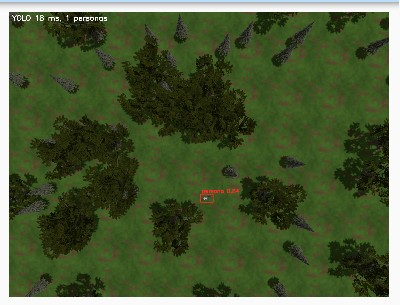
\includegraphics[width=0.55\textwidth]{panel_yolo_personas.jpg}
\caption{Lo que entrega YOLO durante el vuelo: el recuadro rojo con la clase ``persona'' y su
confianza.}
\end{figure}

\section{Cómo se mide si funciona}

\begin{figure}[H]
\centering
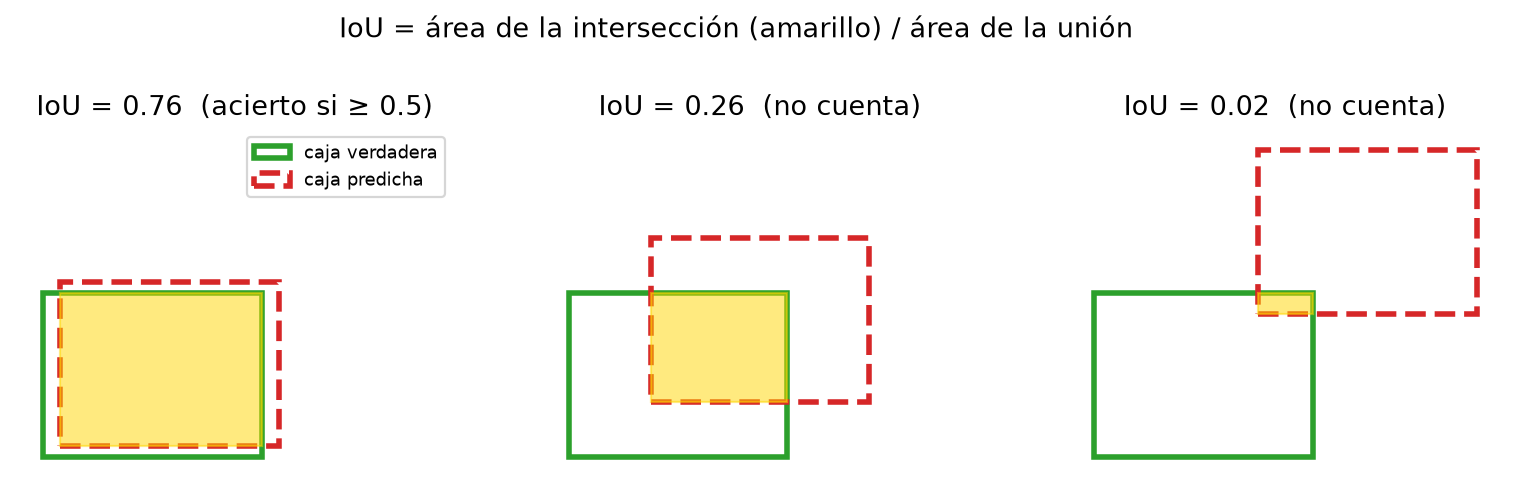
\includegraphics[width=\textwidth]{c_iou.png}
\caption{IoU: intersección sobre unión de la caja predicha y la verdadera.}
\end{figure}

\begin{description}
  \item[Verdadero positivo:] dijo ``persona'' y había una (con IoU $\ge$ 0.5).
  \item[Falso positivo:] dijo ``persona'' y no había (por ejemplo, la sombra de un roble).
  \item[Falso negativo:] había una persona y no la vio.
\end{description}
\begin{align}
\text{precisión} &= \frac{VP}{VP + FP} && \text{(cuando dice ``persona'', ¿cuántas veces acierta?)}\\
\text{recall} &= \frac{VP}{VP + FN} && \text{(de las personas que hay, ¿cuántas encuentra?)}
\end{align}
La \textbf{mAP50} resume la curva precisión-recall con IoU $\ge$ 0.5; la \textbf{mAP50-95} exige además
cajas más ajustadas.

\begin{ejemplo}
En una búsqueda, perder a una persona (falso negativo) es mucho peor que revisar una sombra (falso
positivo). Por eso el umbral de confianza del detector es bajo (0.25) y la misión decide después,
juntando varias detecciones, qué candidatas son confiables.
\end{ejemplo}
